\chapter{Implementation and Experimental Setup}\label{chapter:pipeline}

In this chapter, we will describe the pipeline we have set up to generate constructed languages. The codebase is built in Python, and we used Poetry
for Dependency Management. The pipeline is modular, to allow us to perform ablation studies.

\section{Pipeline Overview}
In order to generate constructed languages, we setup a modular pipeline. Figure~\ref{fig:pipeline_structure} shows the Structure of a generation pipeline.
Although we ended up having the modules in a specific order, the codebase is flexible enough that we can reorder modules, as long as the input to any module has all the features required for its execution. 
This is facilitated by the \texttt{LanguageDescription} class, which contains all the features of a language. This class is piped through the modules,
and each module can add or modify features of the language. Each module also generates a results \texttt{dict} which is stored as a \texttt{JSON} file after the run. 
If the module requires a certain element of the description to be generated beforehand, it check for those features and can throw an error if they are not present.

\begin{figure}
    \centering
    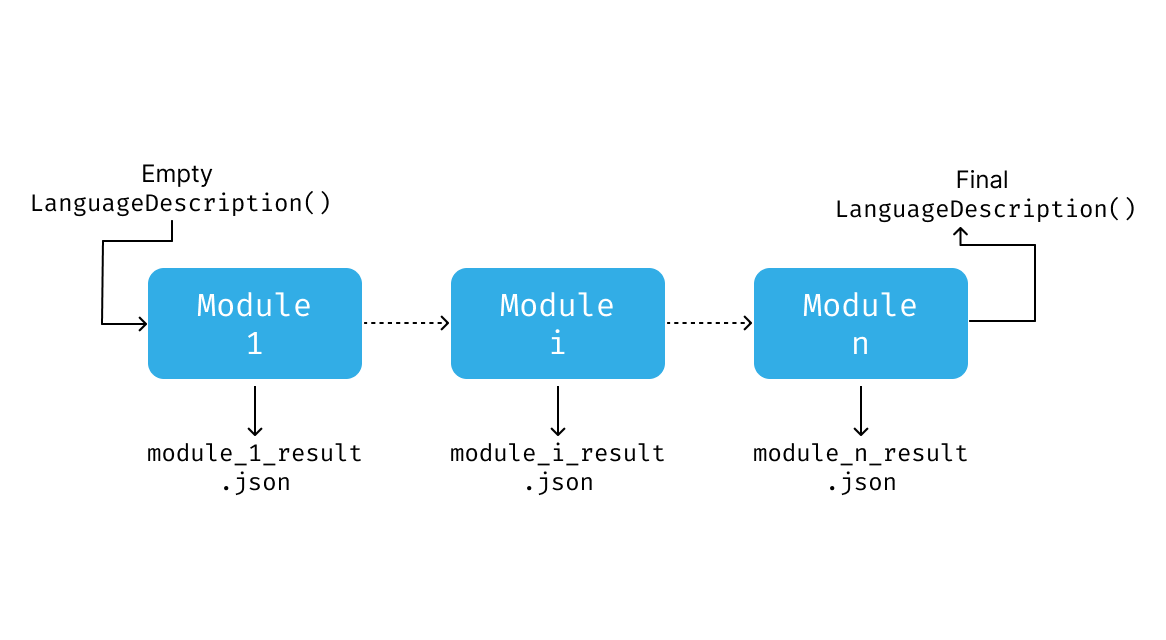
\includegraphics[width=0.8\textwidth]{figures/pipeline_structure.png}
    \caption{The pipeline structure for generating constructed languages. The modules are run in order, and each module can add or modify features of the language.}
    \label{fig:pipeline_structure}
\end{figure}

A pipeline can be setup by subclassing the \texttt{Pipeline} class, which takes care of executing the modules and saving the results. Each module of the pipeline 
is a subclass of the \texttt{Module} class, which has an \texttt{execute} method that takes a \texttt{LanguageDescription} object and other optional arguments,
and returns the modified \texttt{LanguageDescription} object and other optional results.

During the course of development, we found ourselves using more or less similar modules in most of our experiments. We have identified the following modules that are common to most
setups:

\subsection{Phonetics Modules}

The goal of a Phonetics Module is to generate the phonemic inventory of the language. The module configures the \texttt{PhonemeDataInventory} class, which
contains a list of \texttt{PhonemeData}. The phoneme segments for this class are based on PHOIBLE \cite{phoible} segments, with a \texttt{GlyphID} corresponding
to their database. For our purposes, we also implemented an \texttt{alphabet} attribute, to have a simpler representation for phonemes that are
hard to read or write. This was useful for debugging and visualization purposes.

\subsection{Phonotactics Modules}
The goal of a Phonotactics Module is to generate the phonotactic rules of the language. The module configures the \texttt{PhonotacticData} class, which
specifies the rules for syllable structure and phonotactic constraints for word beginnings and endings.

\subsection{Syllable Builder Module}
The Syllable builder modules combines the phonemes generated by the Phonetics Module and the phonotactic rules generated by the Phonotactics Module to
generate all the possible syllables in the language.

\subsection{Grammar Modules}
% TODO

\subsection{Vocabulary Modules}
The goal of the Vocabulary Module is to generate the vocabulary of the language. The module configures the \texttt{VocabDictionary} class, which
holds the list of \texttt{VocabularyEntry} objects. Each \texttt{VocabularyEntry} object contains the word in the constructed language, its translation,
and its definition in english. 
A source words list is also part of each entry, to facilitate easy search for translation purposes. The class can also hold embeddings for each word, which could be also used for downstream tasks.

\subsection{Translation Modules}
Once the language description is generated, we use a translation module to translate some text corpora represented by \texttt{AbstractSourceText}.
The module translates the source text paragraph by paragraph, using an LLM model.

\subsection{Evaluation Modules}
Figure~\ref{fig:evaluations_structure} shows the setup for running evaluations on the generated languages. The Evaluators are a separate class 
that does not inherit from the abstract \texttt{Module} class. They inherit the \texttt{Evaluator} class, which creates an evaluations folder 
inside the results folder, to store the results of the evaluations. 

\begin{figure}
    \centering
    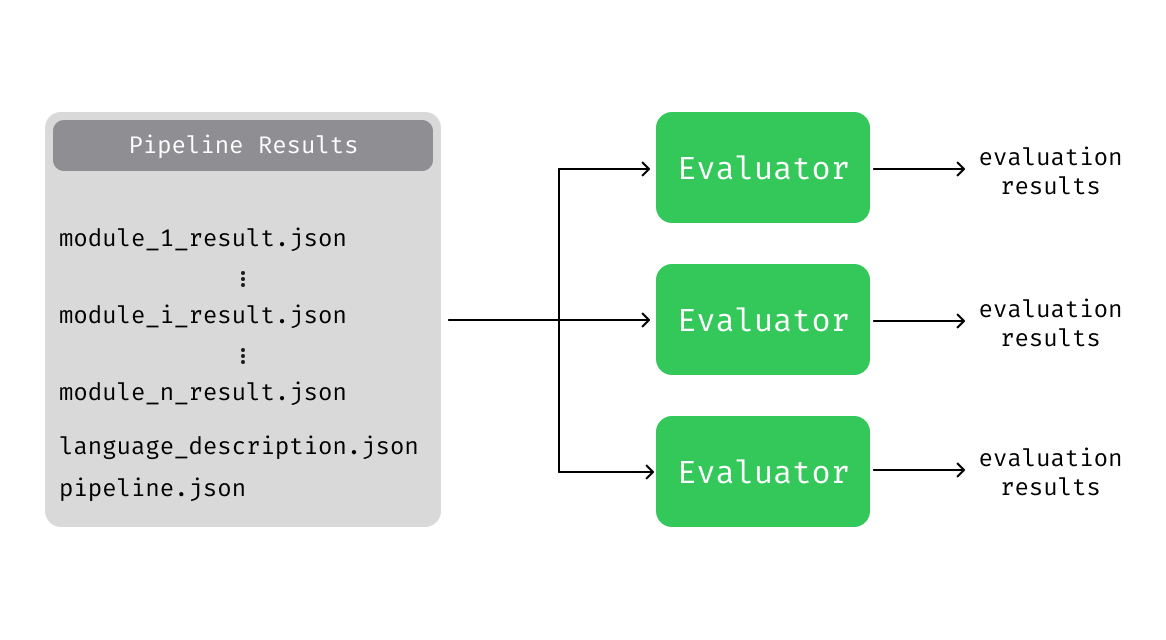
\includegraphics[width=0.8\textwidth]{figures/evaluations_structure.png}
    \caption{The setup for running evaluations. Each evaluator stores the results in a folder inside the evaluations folder.}
    \label{fig:evaluations_structure}
\end{figure}